\section{Aufbau}
\label{sec:Aufbau}

Es wird ein Kreislauf aufgebaut, in dem ein Wasser-Glycerin-Gemisch mit Glaskugeln durch Rohre und Schläuche strömt. (siehe \autoref{fig:foto_aufbau})

\begin{figure}
    \centering
    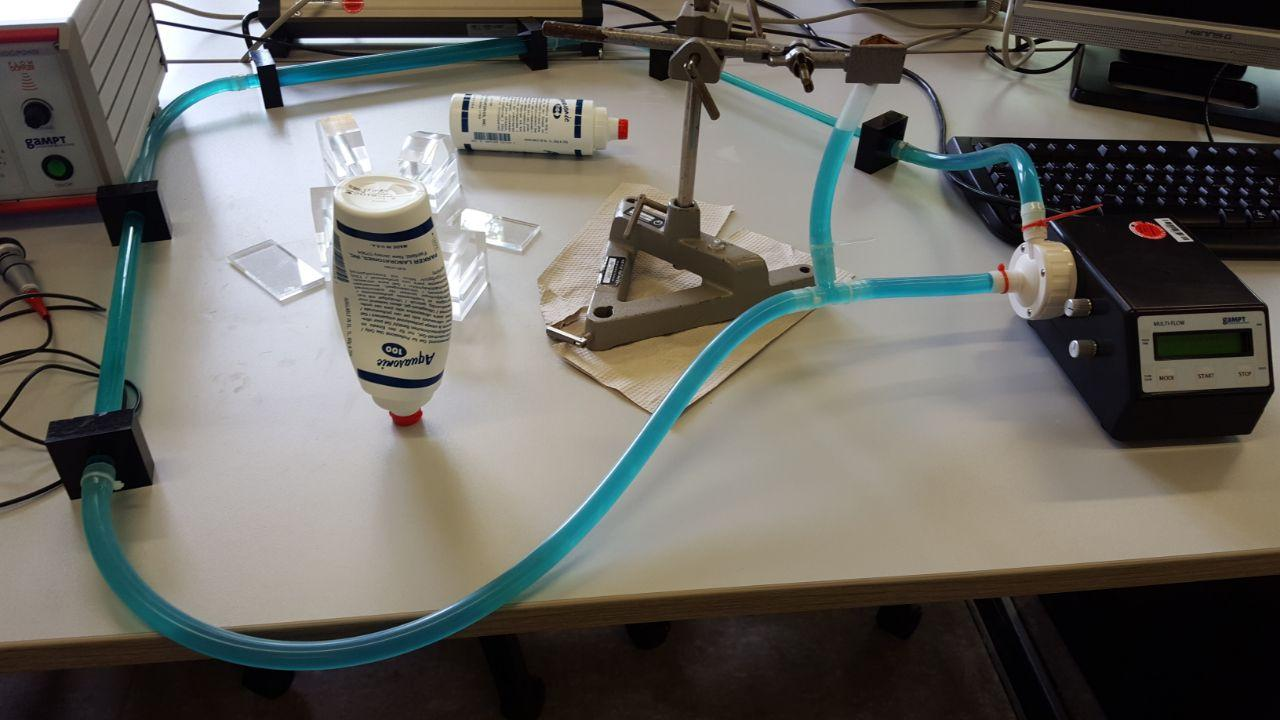
\includegraphics[width=0.8\textwidth]{images/foto_1.jpg}
    \caption{Foto des Kreislaufs bzw. des Versuchaufbaus}
    \label{fig:foto_aufbau}
\end{figure}

An einer Stelle des Kreislaufs wird die Flüssigkeit untersucht.
Das Rohr an dieser Stelle besteht aus Acryl und hat einen Innenradius von $R_i=\SI{5}{\milli\metre}$ und einen Außenradius von $R_a=\SI{7.5}{\milli\metre}$.
Die Flüssigkeit wird von einer Zentrifugalpumpe angetrieben, an welcher die Fließgeschwindigkeit einstellbar ist.

\FloatBarrier

\begin{figure}
    \centering
    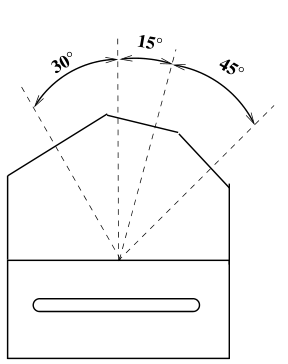
\includegraphics[width=0.2\textwidth]{images/skizze_2.png}
    \caption{Skizze des verwendeten Doppler-Prismas \cite{US3}}
    \label{fig:skizze_prisma}
\end{figure}

Um die Schallsonde in einem vorbestimmten Winkel $\theta$ mit dem Rohr zu koppeln wird ein Doppler-Prisma wie in \autoref{fig:skizze_prisma} verwendet.
Dieses ist ebenfalls aus Acryl.
Die Abstände der Flächen zum Rohr sind alle $l=\SI{30.7}{\milli\metre}$.
Da Acryl und die hier verwendete Flüssigkeit verschiedene Dichten haben, wird der Schall an der Grenzfläche gebrochen und im Allgemeinen ist $\alpha \neq \theta$.
Der tatsächliche Einschallwinkel wird über
\begin{equation}
    \alpha = \SI{90}{\degree} - \arcsin \left( \sin \theta \cdot \frac{c_F}{c_A} \right)
    \label{eq:dopplerwinkel}
\end{equation}
berechnet, wobei $c_F$ die Schallgeschwindigkeit in der Flüssigkeit und $c_A$ die Schallgeschwindigkeit in Acryl ist.


Als Schallsender und -empfänger wird hier eine $\SI{2}{\mega\hertz}$ Schallsonde verwendet.
Diese wird an einen Doppler-Generator angeschlossen, welcher mit einem Computer verbunden ist.
Die gemessenen Daten werden am Computer mit dem Programm FlowView dargestellt und ausgewertet.

Das Doppler-Prisma wird mit einem Ultraschall-Gel an das Rohr gekoppelt, da Luft ein hohen Schallabsorption aufweist.


\section{Durchführung}
\label{sec:Durchführung}

Im ersten Teil des Versuchs wird die Strömungsgeschwindigkeit durch das Acrylrohr für fünf verschiedene Geschwindigkeiten bestimmt. 
Diese Messung wird an allen drei Doppler-Winkeln wiederholt. (siehe \autoref{fig:skizze_prisma})

Dazu wird die Sonde mit Ultraschall-Gel am Doppler-Prisma gekoppelt.
Am Doppler-Generator wird ein Sample-Volume von Large eingestellt.
An der Pumpe wird eine Strömungsgeschwindigkeit eingestellt und als Vergleichswert notiert.
Dann wird am Computer die durchschnittliche Frequenzverschiebung abgelesen und notiert.

Im zweiten Teil des Versuchs wird das Strömungsprofil der Doppler-Flüssigkeit bestimmt.

Dazu wird die Sonde am Doppler-Prisma mit $\theta=\SI{15}{\degree}$ gekoppelt.
Das Sample-Volume wird auf Small gestellt.
An der Pumpe wird eine Strömungsgeschwindigkeit von $\SI{70}{\percent}$ der maximalen Geschwindigkeit eingestellt.
Eine zweite Messreihe wird mit einer Pumpleistung von $\SI{35}{\percent}$ durchgeführt.

Nun kann am Doppler-Generator die Messtiefe eingestellt werden.
Diese wird in $\si{\micro\second}$ angegeben, wobei dies der Zeit entspricht, die die Schallwelle benötigt um durchs Medium zu laufen bis sie reflektiert wird.
Es soll der gesamte Rohrdurchmesser durchlaufen werden, also muss zunächst berechnet werden in welchem Messtiefebereich gemessen werden muss.

In Acryl hat Schall eine Geschwindigkeit von 
\begin{equation*}
    c_A \approx \SI{2700}{\metre\per\second} \approx \frac{10}{4}\si{\milli\metre\per\micro\second} \, .
\end{equation*}
Die Schallgeschwindigkeit in der Doppler-Flüssigkeit ist
\begin{equation*}
    c_F \approx \SI{1800}{\metre\per\second} \approx \frac{6}{4}\si{\milli\metre\per\second} \, . \text{\cite{US3}}
\end{equation*}
Also kann die minimale Messtiefe (die Strecke von der Sonde bis zum inneren Rand des Rohrs) über
\begin{equation}
    d_\text{min} = \frac{l+R_a-R_i}{c_A}
    \label{eq:messtiefe_min}
\end{equation}
und die maximale Messtiefe (die Strecke von der Sonde bis zum inneren Rand des Rohrs auf der anderen Seite) über
\begin{equation}
    d_\text{max} = d_\text{min} + \frac{2 \cdot R_i}{c_F}
    \label{eq:messtiefe_max}
\end{equation}
berechnet werden.
Damit ergibt sich ein sinnvoller Bereich der Messtiefe von $\SI{12.5}{\micro\second}$ bis $\SI{19.5}{\micro\second}$.
In einem Abstand der Messtiefe von $\SI{0.5}{\micro\second}$ werden die maximal gemessenen Frequenzverschiebungen und die gemessenen Schallintensitäten am Computer abgelesen und notiert.